\section{Software description}

\subsection{Software components}

\subsubsection{preCICE}
\begin{itemize}
	\item An overview is shown in Figure \ref{fig:precice:overview}
	\item Coupled simulation programs are called \textit{solvers} or \textit{participants}
	\item preCICE connects different solvers to perform a partitioned simulation
	\item preCICE takes care of different coupling aspects such as data mapping and communication
	\item Different coupling schemes can be implemented: Who is coupled o whom, what data is exchanged, which coupling algorithms are used \cite{Gatzhammer:2014}
	\item Multi-coupling: Couple multiple (in theory: arbitrary many) participants in different configurations (explicit, implicit)
	\item Acceleration: Use acceleration algorithms to reach a decent computation time
	\item Time interpolation: Use solvers with different time step sizes
	\item Coupling scheme is defined in the precice-config.xml, the only global file which is accessed by all participants
	\item For each solver, a specific \textit{adapter} is necessary to communicate to preCICE
	\item Adapter is an additional piece of software
	\item Adapter can take many forms depending on the solver, eg.: OpenFOAM - C++ Function object, FEniCS - Python module
	\item Different Language bindings are available: C/C++, Python, Fortran, Julia, Matlab
	\item The Adapter allows the solver to access preCICE and to call the coupling
\end{itemize}

\begin{figure*}[t]
	\centering
	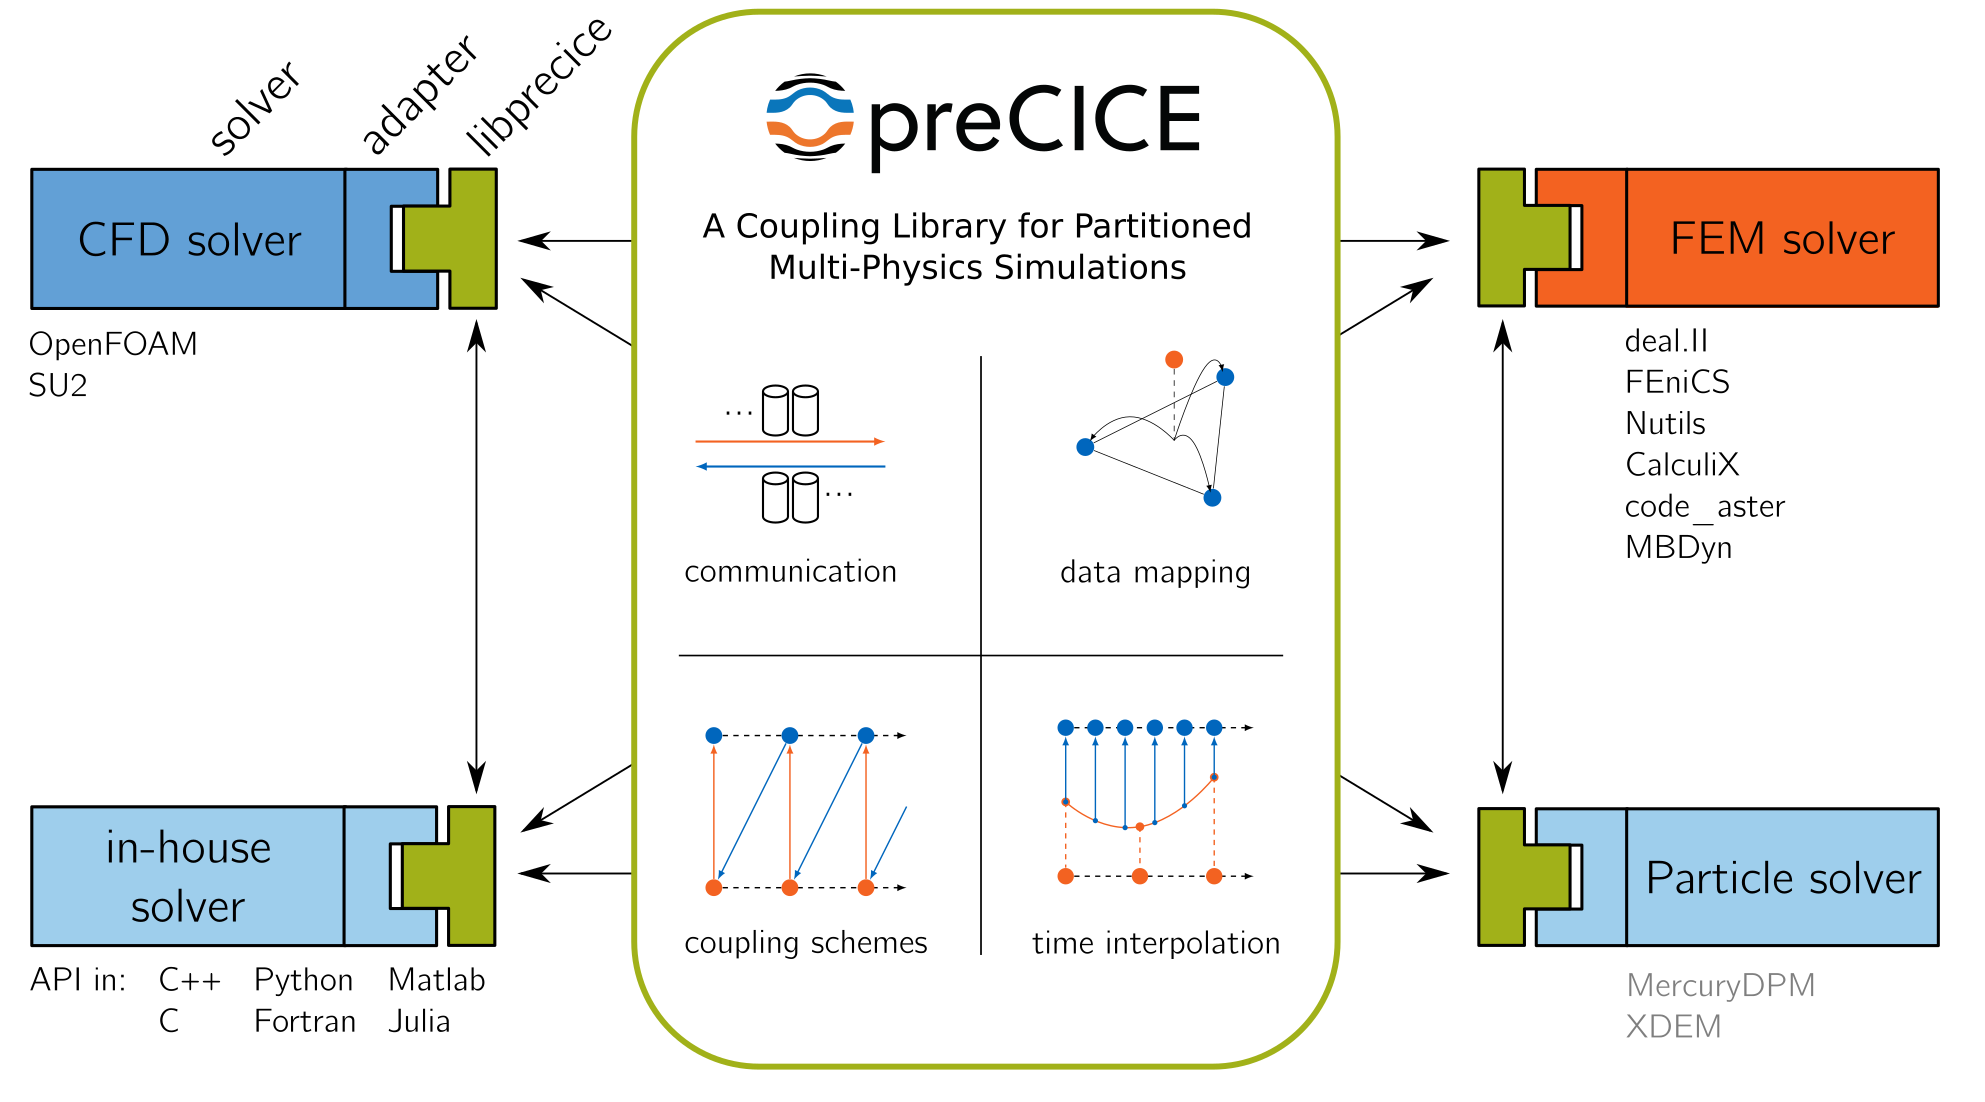
\includegraphics[width=0.9 \textwidth]{images/precice-overview.png}
	\caption{preCICE overview \cite{Chourdakis:2022}}
	\label{fig:precice:overview}
\end{figure*}


\subsubsection{OpenFOAM and the preCICE-OpenFOAM adapter}
\begin{itemize}
	\item OpenFOAM
	\begin{itemize}
		\item Popular open-source PDE tool in academia and industry
		\item Enables the use and modification of different solvers
		\item Used mainly for CFD but also FEM simulations 
	\end{itemize}
	\item Adapter
	\begin{itemize}
		\item Enables the coupling of OpenFOAM via preCICE in different simulation scenarios
		\item Exemplifies the development strategy behind preCICE: Adapter is a library for OpenFOAM and called on runtime to perform the coupling without any modification to the OpenFOAM source code
		\item Different modules for different kinds of multi-physics simulations: FSI, FF, CHT
	\end{itemize}
\end{itemize}	
Note:
I should introduce the OpenFOAM adapter at some point.
Lets introduce the broad concept of the adapter here and add more details, eg about the specific files that would need to be modified, later in the Challenges part
\newline
\subsubsection{OpenFAST}
\begin{itemize}
	\item Wind energy engineering tool developed by NREL
	\item Widely used in academia and industry
	\item Simulates the coupled aerodynamic, structural, and electrical behaviour of wind turbines as well as the control response
	\item Allows to model on- and offshore wind turbines and can be used to compute wind parks as well
	\item OpenFAST is a glue code for different modules which compute the various physical domains
	\item Takes one main input file denoted \textit{.fst} which points to more specific files for each computation module (eg AeroDyn, ServoDyn, ...)
	\item Fidelity: Does OpenFAST include computations in different fidelities? Is it a low- to mid-fidelity tool?
	\item Computes the Fluid-Structure-Interaction at blades and tower with the actuator line method
	\item Inflow field is either computed by AeroDyn or received from external CFD solver
	\item Has a dedicated C++ API for the coupling with CFD solvers
\end{itemize}

OpenFAST is mainly used to perform turbine loads analysis and drive the detailed turbine design. The computational cost is therefore higher than for tools used in the early design exploration phase like WISDEM, RAFT or FLORIS, but lower than highly resolved solvers necessary to understand the actual physics and check the final turbine design like ExaWind or SOWFA. 

\subsection{Software concept}

Main idea
\begin{itemize}
	\item Write a preCICE-OpenFAST adapter (see Figure \ref{fig:setup}), a new piece of software that connects OpenFAST and preCICE
	\item Acts as driver code towards OpenFAST: Calls it via the C++ API
	\item Calls preCICE to communicate data and steering commands
	\item Configurable by two .yaml input files
	\item preciceSettings.yaml contains information about the coupling setup
	\item openfastSettings.yaml contains information about the turbine simulation case
	\item The concept is sketched out in Figure \ref{code:adapter}
	\item line 8-10: Instantiate and initialize the interface to OpenFAST
	\item line 12-14: Do the same for preCICE
	\item Now both software component are ready to use
	\item line 16: main time loop controlled by preCICE
	\item line 18: Read velocity data from CFD solver via preCICE and store it in local variable
	\item line 20: Set the velocity data in OpenFAST
	\item line 22: Tell OpenFAST to compute the wind turbine dynamics for the next time step
	\item line 24: Get the resulting force from OpenFAST and store it in local variable
	\item line 26: Send force data to CFD solver to be used in ALM method
	\item line 28: Advance both solvers in time
	\item line 30-31: End the simulation after the main loop has finished
	\item Developed and documented on GitHub\footnote{\url{https://github.com/LeonardWilleke/openfast-adapter}}\\
\end{itemize}

\begin{comment}
	The OpenFAST adapter is something between the FMI Runner and a normal adapter:
	It executes OpenFAST like the runner but OpenFAST is a full, executable program on
	its own.
	
	\begin{figure*}[t]
	\centering
	\includegraphics[width=0.9 \textwidth]{images/precice-openfast-adapter-setup.png}
	\caption{preCICE-OpenFAST Adapter software architecture}
	\label{fig:openfast:adapter}
	\end{figure*}
\end{comment}


\begin{figure}[h!]
	\centering
	\begin{minipage}{0.9\textwidth}
		\begin{minted}{cpp}
		#include <OpenFAST.H>
		#include <precice.hpp>
		
		vector<double> readData;
		vector<double> writeData;
		
		// OpenFAST Setup
		fast::OpenFAST FAST;
		...
		FAST.init()
		// preCICE Setup
		participant = precice.participant(...);
		...
		participant.initialize();
		// main time loop
		while participant.isCouplingOngoing(): 
			// Get read data from preCICE
			participant.readData(readData, ...);
			// Set read data in OpenFAST
			FAST.setVelocity(readData, ...);
			// Compute next time step
			FAST.step();
			// Get write data from OpenFAST
			FAST.getForce(writeData, ...);
			// Send write data to preCICE
			participant.writeData(writeData, ...);
			// Advance preCICE in time
			participant.advance(dt) 
		
		participant.finalize()
		FAST.end()
		\end{minted}
	\end{minipage}
	\caption{Concept of the OpenFAST adapter: The script utilizes the C++ API to execute OpenFAST and calls preCICE to couple the simulation. For conciseness, API calls are simplified.}
	\label{code:adapter}
\end{figure}
